\chapter{Métodos Iterativos}
Como ya hemos visto, los métodos directos poseen en general una complejidad de orden cúbico en el número de incógnitas $\mathcal{O}(N^3)$. Esto dice que si en un problema determinado se duplica el número de incógnitas entonces el número de operaciones se multiplica por 8. Eso ha llevado a intentar desarrollar métodos de orden menor \footnote{Observe que el límite inferior para un método de resolución  es $\mathcal{O}(N^2)$ ya que ese es el número de coeficientes de la matriz.} y los métodos iterativos son una posible alternativa.

Hay, además de la complejidad,  otros problemas con los métodos directos. Por ejemplo, en muchas aplicaciones aparecen problemas con un número muy grande de incógnitas pero con matrices \emph{ralas}, es decir, matrices con un elevado porcentaje de coeficiente nulos. Esto permite en principio reducir notablemente el número de operaciones del algoritmo pero sin embargo como desventaja aparece un ``rellenado'' innecesario en la factorización resultante. En la siguiente sección vemos un ejemplo sencillo.

\section{Un ejemplo: distribución de temperatura}
\label{sec:piston}
Ciertas ecuaciones diferenciales lineales  pueden resolverse de modo aproximado a través de \emph{discretizaciones}.
En dimensión uno es fácil imaginar como puede hacerse. Por ejemplo, la distribución estacionaria de la temperatura a lo largo de una barra o alambre se modeliza (sin  tener en cuenta las constantes físicas) a través de la ecuación
$$
u''(x)=f(x),
$$
donde $u(x)$ representa la temperatura en de la barra en el punto $x$ y $f(x)$ una fuente de calor. Si asumimos que la barra ocupa un intervalo $[a,b]\subset \R$ podemos tomar puntos equiespaciados sobre la barra
$a=x_0<x_1<\cdots <x_{n+1}=b$ definidos como $x_i=a+ih$ donde $h=\frac{b-a}{n+1}$. Cuando $n\to \infty$ (aumentamos el número de puntos) resulta que $h\to 0$ y como\footnote{Usar Taylor para verficar la última identidad.}
$$
\frac{u(x_{i+1})-2u(x_i)+u(x_{i-1})}{h^2}=
\frac{u(x_{i}+h)-2u(x_i)+u(x_{i}-h)}{h^2}=
u''(x_i)+\mathcal{O}(h^2),
$$
vemos que podemos aproximar la temperatura en el punto $x_i$ resolviendo
$$
u(x_{i+1})-2u(x_i)+u(x_{i-1})=f(x_i)h^2,
$$
lo que conduce a un sistema (una ecuación por cada $x_i$) \emph{tridiagonal} que en este caso simplificado se escribe
$$\begin{pmatrix}
-2&1&0&0&\cdots &0&0\\
1&-2&1&0&\cdots &0&0\\
0&1&-2&1&\cdots &0&0 \\
\vdots&\vdots&\vdots&\vdots&
\cdots &\vdots&\vdots\\
0&0&0&0&\cdots& 1&-2
\end{pmatrix}
\begin{pmatrix}
 u(x_1)\\
 u(x_2)\\
 \vdots\\
 u(x_n)
 \end{pmatrix}=
 \begin{pmatrix}
 f(x_1)\\
 f(x_2)\\
 \vdots\\
 f(x_n)
 \end{pmatrix}.
$$
En dimensión mas alta (por ejemplo en dimensión 3) el problema de la difusión del calor se modeliza con la ecuación
$$
\Delta u(x)=f(x),
$$
donde $\Delta u(x)=u_{xx}(x)+u_{yy}(x)+u_{zz}(x)$ representa al Laplaciano de $u$. Para ver un ejemplo concreto en la Figura \ref{fig:disc_piston} se muestra un cuarto de pistón (pieza que se desplaza dentro de uno de los cilindros de un motor). La distribución de temperatura en esa pieza puede aproximarse resolviendo una discretización la ecuación del calor.
\begin{figure}[h]
\centering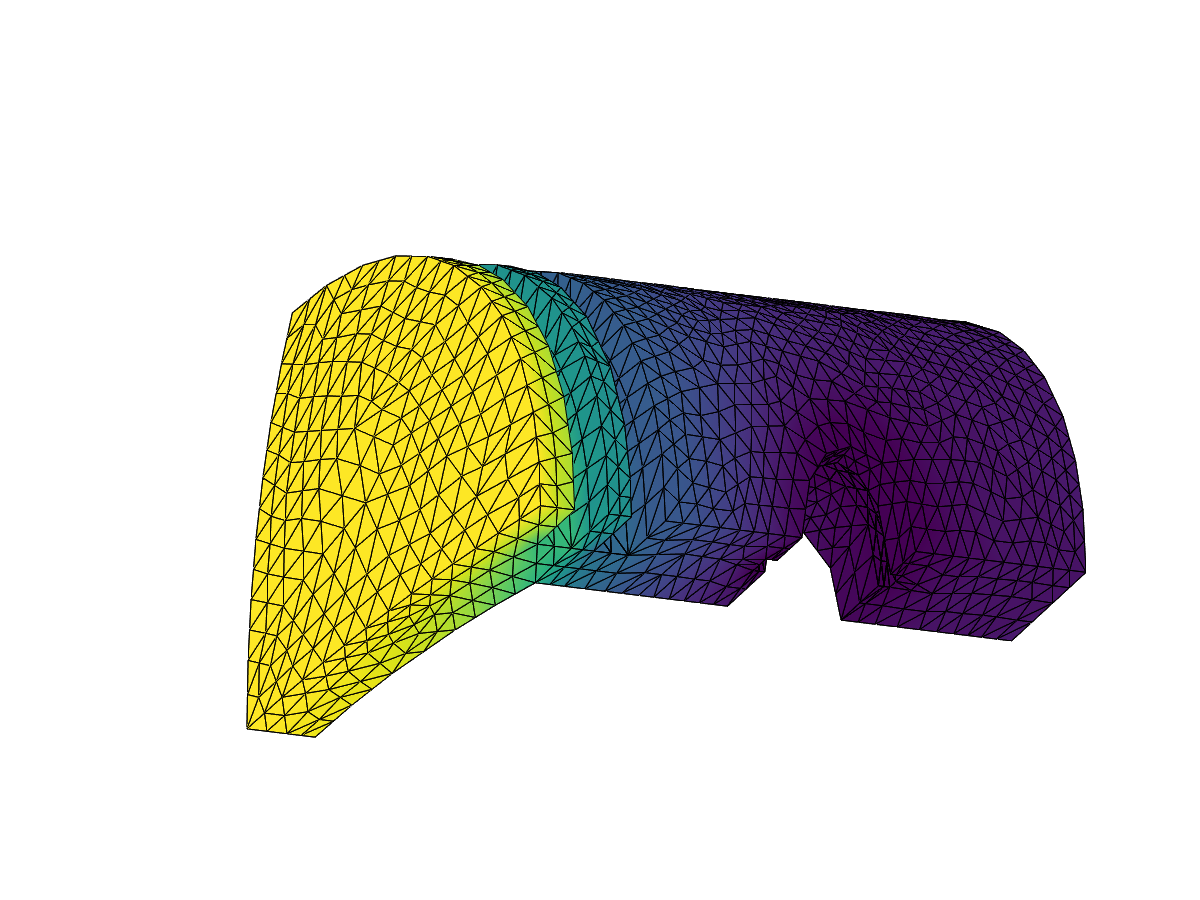
\includegraphics[width=0.3\linewidth]{piston.png}
\label{fig:disc_piston}
\caption{Distribución de temperatura en un pistón. Se visualiza un cuarto de la pieza.}
\end{figure}
No vamos a describir aquí como hacer esto, pero una vez discretizado, el problema puede escribirse como un sistema lineal de ecuaciones\footnote{La discretización de ecuaciones diferenciales \emph{lineales} conduce a sistemas lineales.}. En este ejemplo particular, el sistema resultante  puede escribirse de la forma
 $$
 \Ab\xb=\bb,
 $$
 donde
 $$\Ab\in \R^{3319\times 3319}$$
cada incógnita es el valor de la temperatura en un punto interior del pistón. Este ejemplo que llamaremos $(E)$ nos servirá para ejemplificar algunas particularidades que aparecen en este capítulo. En este problema aparece una propiedad que puede verse en muchas otras aplicaciones: la matriz resulta rala\footnote{ En inglés sparse: un porcentaje significativo de elementos de la matriz es nulo.} además de \emph{simétrica}. En la Figura \ref{fig:matrizA}
\begin{figure}[h]
\label{fig:matrizA}
\centering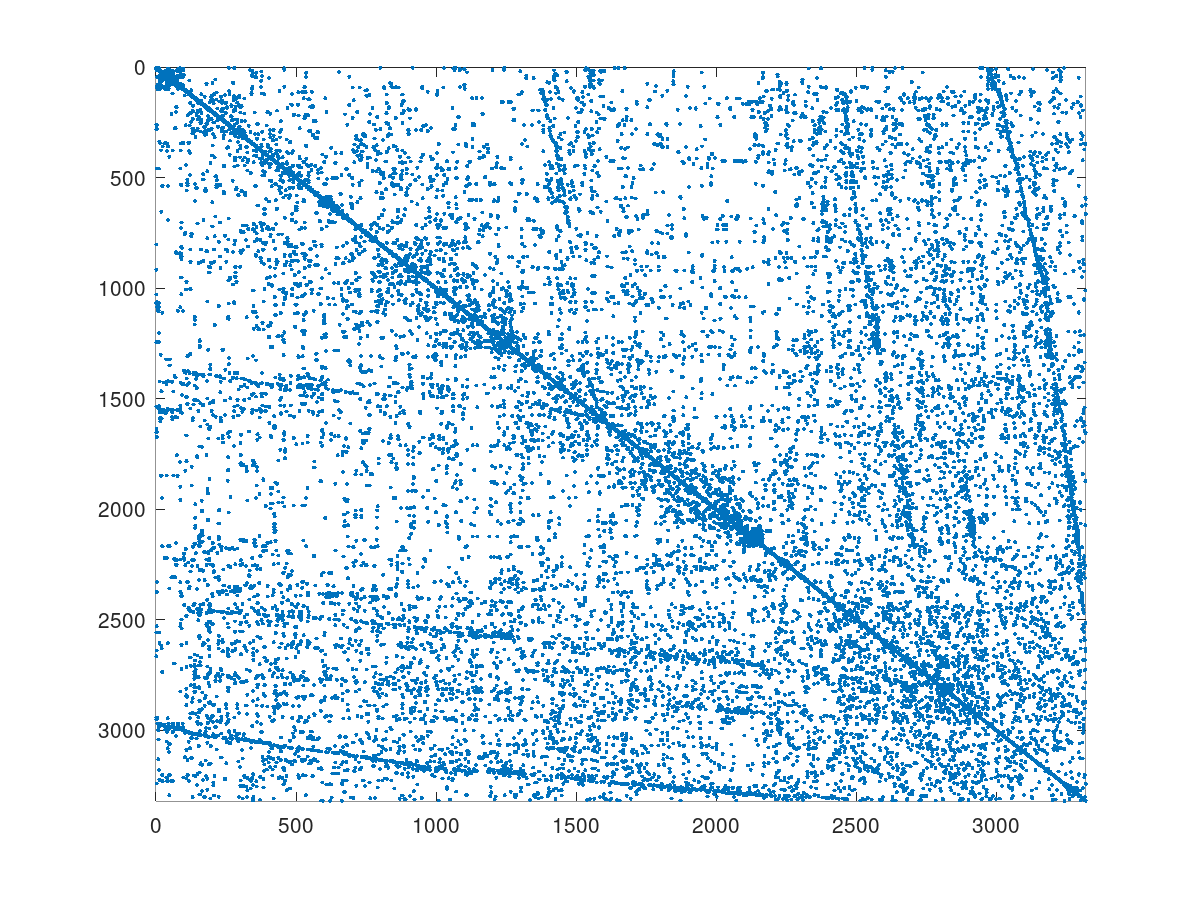
\includegraphics[width=0.4\linewidth]{matrizA.png}
\caption{Estructura de la matriz $A$: se observa que es rala y simétrica.}
\end{figure}
se observan ambos hechos (con el comando np.spy(A)). En este caso, solamente $39753$ coeficientes son diferentes de cero, en vez $3319^2=11015761$ que representan el total de elementos de la matriz. Desde  el punto de vista de la memoria utilizada en el almacenamiento de $\Ab$ esto es significativo. Teniendo en cuenta que en doble precisión cada número ocupa 8 bytes tendriamos en cada caso:
\begin{itemize}
 \item $39753\frac{8}{1024}\sim 300K$
 \item $11015761 \frac{8}{(1024)^2}\sim 84M$.
\end{itemize}
Esta ventaja se puede perder al hacer $LU$.
En efecto, en este ejemplo, a pesar de que $A$ tiene solo $39753$ elementos no nulos, el número de elementos no nulos de $L$ es $2440542$ ($\sim 18M$). Este fenómeno se conoce como \emph{rellenado}. La apariencia de $L$ y su comparación con la matriz original puede verse en la Figura \ref{fig:LyA}

\begin{figure}[h]
\centering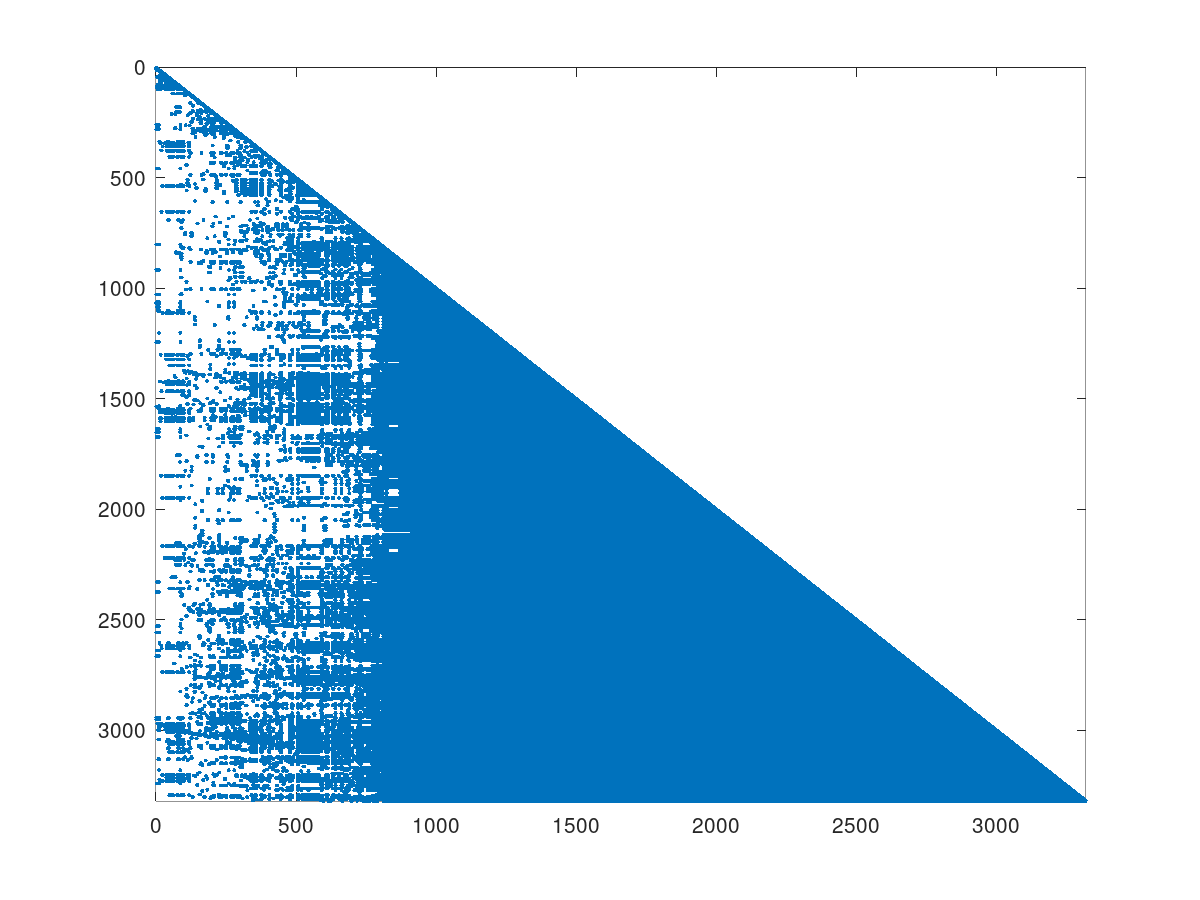
\includegraphics[width=0.3\linewidth]{matrizL.png}
\centering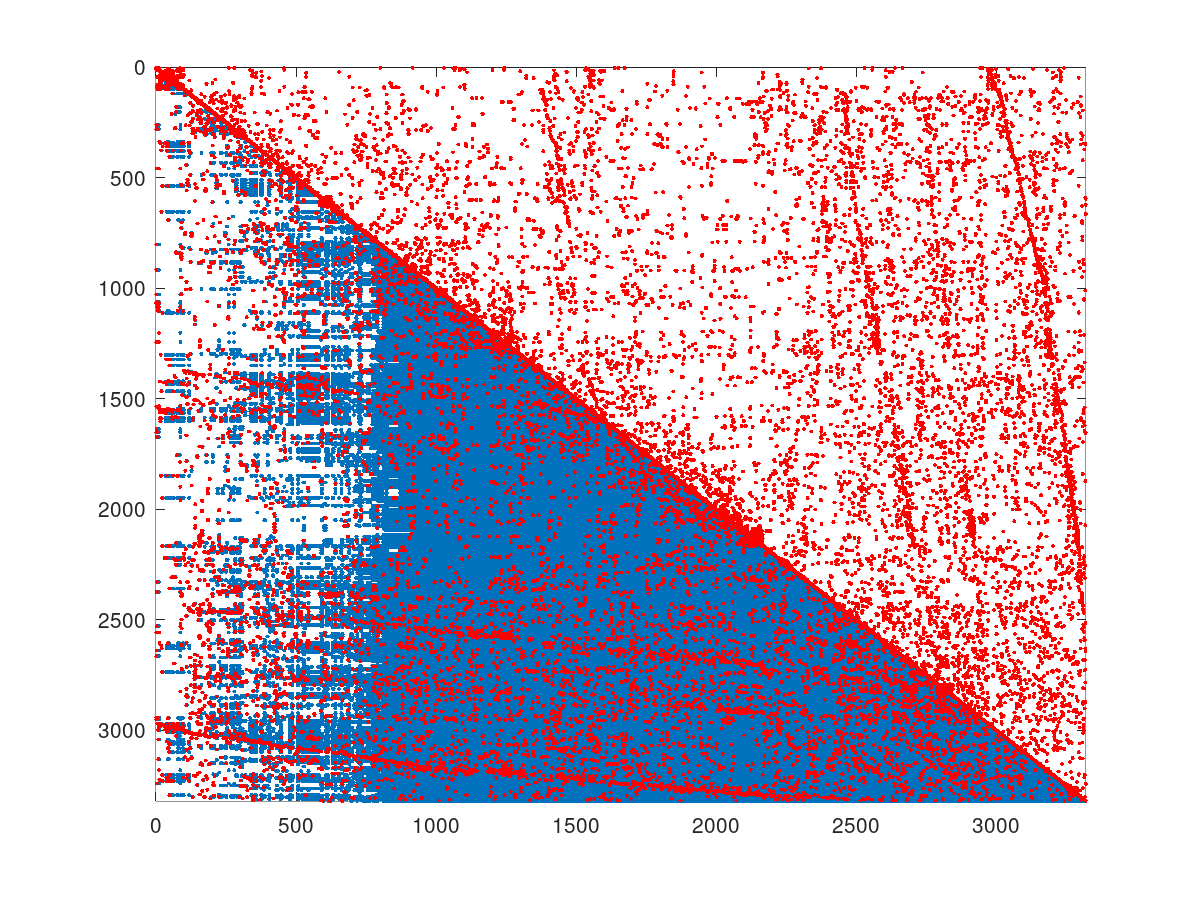
\includegraphics[width=0.3\linewidth]{matricesAyL.png}
\label{fig:LyA}
\caption{Estructura de las matrices $A$ y $L$ en el ejemplo $(E)$. Izquierda, matriz $L$ de la factorización $A=LU$ donde se nota el rellenado. Derecha, superposición de $A$ y $L$.}
\end{figure}


Si bien hay heurísticas para evitar el rellenado, buscando permutar las variables y las ecuaciones no las vamos a comentar en este texto. Vamos a concentrarnos en los métodos iterativos. Estos no buscan ninguna factorización y se basan en iterar un procedimiento de orden $\mathcal{O}(N^2)$ (básicamente el producto de una matriz por vector)  con el esperanza de conseguir una buena aproximación de la solución buscada en unas pocas \footnote{Pocas al menos relativo al tamaño $N$ de la matriz.} iteraciones. 

Ya hemos visto que $\rho(\Ab)$ no es una norma, sin embargo verifica:
$$
\rho(\Ab)=\inf_{\|\cdot\|} \|\Ab\|.
$$
Lo que implica que para todo $0<\varepsilon$ existe una norma $\|\cdot\|$ tal que
$$\|\Ab\|\le \rho(\Ab)+ \varepsilon$$ Usaremos esta propiedad en la demostración del siguiente resultado que da la clave para predecir el orden de convergencia de los métodos iterativos.
\tcc
\begin{prop}
 Para toda norma subordinada $\|\cdot\|$ vale que
 $$
 \rho(\Mb)=\lim_{k\to \infty} \|\Mb^k\|^{1/k}.
 $$
\end{prop}

\etcc


\begin{proof}
 Dado $\epsilon>0$ existe una norma subordinada $\|\cdot\|_{*}$ tal que
 $$
 \|\Mb\|_{*}\le \rho(\Mb)+\epsilon.
 $$
 $$
 \rho(\Mb)^k=\rho(\Mb^k)\le \|\Mb^k\|\le C \|\Mb^k\|_{*}\le C \|\Mb\|^k_{*}\le C(\rho(\Mb)+\epsilon)^k,
 $$
 $$
 \rho(\Mb)\le \|\Mb^k\|^{1/k}\le C^{1/k}(\rho(\Mb)+\epsilon)
 $$
 tomando límite y notando que $\epsilon$ es arbitrario se demuestra el resultado.
\end{proof}
\section{Métodos Iterativos}
Supongamos que queremos resolver
$$
\Ab\xb=\bb,
$$
pero la matriz $\Ab$ es difícil de invertir. Entonces proponemos una descomposición
$$\Ab=\Bb+\Cb,$$
donde $\Bb$ es elegida de modo que sea \emph{fácil} de invertir y escribimos
$$
\Bb\xb=-\Cb\xb+\bb,
$$
o equivalentemente
$$
\xb=-\Bb^{-1}\Cb\xb+\Bb^{-1}\bb.
$$
Notemos que llamando $\Mb_I=-\Bb^{-1}\Cb$  (denominada \emph{matriz de iteraciones}) y $\Bb^{-1}\bb=\tilde{\bb}$,  resolver el sistema equivale a hallar $\xb$ tal que
$$
\xb=\Mb_I\xb+\tilde{\bb}.
$$
La idea es tomar un vector inicial $\xb_0$ e iterar
$$
\xb_{n+1}=\Mb_I\xb_n+\tilde{\bb},
$$
con la esperanza de que $\xb_k\to \xb$. Para ver si nuestra idea puede funcionar estudiamos el error $\eb_k=\xb-\xb_k$ restando miembro a miembro las dos ecuaciones de arriba
$$
\eb_{k+1}=\Mb_I\eb_k=\Mb_I\Mb_I\eb_{k-1}=\cdots = \Mb^{k+1}_I\eb_0
$$
de donde vemos que $\eb_k\to \cero$ para \emph{todo} error inicial $\eb_0$ sí y solo sí
$\Mb_I^{k}\to \cero $ lo cual ocurre sí y solo sí $\rho(\Mb_I)<1$.

Más aún
$$
\|\eb_k\|\le C\rho(\Mb_I)^k
$$
lo que nos da la velocidad de convergencia del algoritmo.

Comencemos estudiando un caso particular llamado el método de Richardson.
 Elegimos $\Bb$ como un múltiplo de la identidad
$$\Bb=\omega^{-1}\Ib, \qquad \omega>0.$$
Luego, se tiene
$$\Cb=\Ab-\omega^{-1}\Ib=\omega^{-1}(\omega\Ab-\Ib)$$
y la matriz de iteraciones resulta
$$
\Mb_I=-\Bb^{-1}\Cb=
\Ib-\omega\Ab
$$

\tcc
\begin{prop}
Si $\Ab$ es SDP, el método de Richardson converge -para todo dato inicial- sí y solo sí $\omega<\frac{2}{\rho(\Ab)}.$
\end{prop}
\etcc

\begin{proof}
 Basta ver bajo que condiciones $\rho(\Mb_I)<1$, con $
\Mb_I=
\Ib-\omega\Ab.
$ Como $\Ab$ es SDP sus autovalores cumplen $0<\lambda_1\le \lambda_2\le \cdots \le \lambda_n$. Los autovalores de $
\Mb_I$ son entonces $1-\omega\lambda_i$.  Queremos ver bajo que condiciones
$
|1-\omega\lambda_i|<1,
$ para todo $1\le i\le n$. Equivalentemente,
$$
-1< 1-\omega\lambda_i< 1
$$
i.e. es necesario y suficiente que $\omega<\frac{2}{\lambda_i}$ para todo $1\le i\le n$ lo que equivale a
$\omega<\frac{2}{\rho(\Ab)}.$
\end{proof}

Claramente, al variar $\omega$ en el rango $(0,\frac{2}{\rho(\Ab)})$ obtendremos distintas velocidades de convergencia para nuestro método. Podemos intentar localizar el óptimo $\omega_{opt}$, es decir el que garantiza orden máximo de convergencia (equivalentemente, el $\omega_{opt}$ para el cual $\rho(\Mb_I)$ es mínimo). Para ello observemos que   (ver Figura \ref{fig:modulos}) como
$$
\rho(\Mb_I)=\max\{
|1-\omega   \lambda_n|,|1-\omega   \lambda_1|\}
$$
$\omega_{opt}$ ocurre en el punto de cruce de los gráficos.
\begin{figure}[h]
\label{fig:modulos}
\centering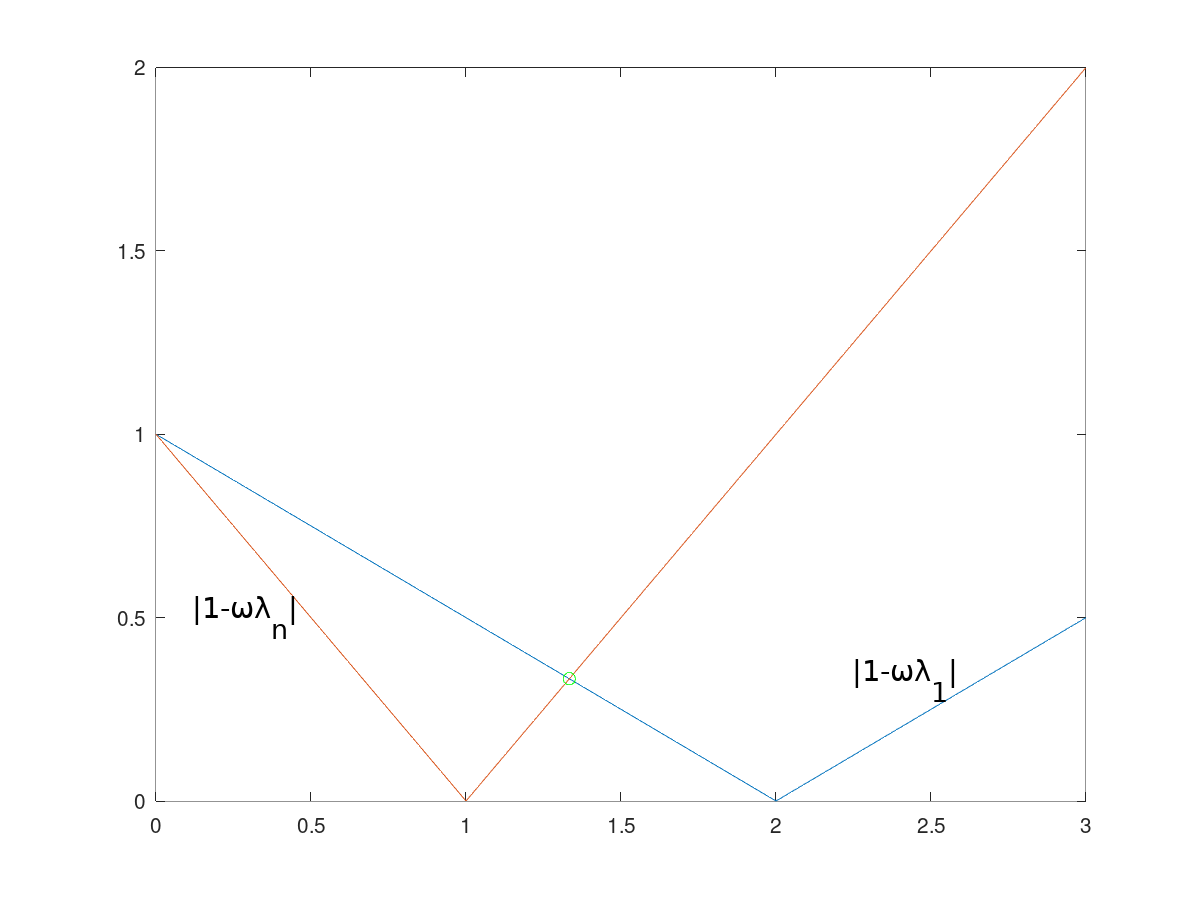
\includegraphics[width=0.4\linewidth]{modulos.png}
\end{figure}
Ese punto puede despejarse 
$$
\omega_{opt}=\frac{2}{\lambda_n+\lambda_1}
$$
de donde el respectivo radio espectral óptimo es 
$$\rho(\Mb_I)=\frac{\lambda_n-\lambda_1}{\lambda_n+\lambda_1}=\frac{\kappa(\Ab)-1}{\kappa(\Ab)+1}.
$$
Notemos que la velocidad de convergencia del método se deteriora si  $\kappa(\Ab)$ es grande.

\tcc
Para el ejemplo $(E)$ de la distribución de temperatura, dado al principio del capítulo, tenemos (aproximados por el método de la potencia)

$$
\lambda_1\sim 0.0009 \qquad \lambda_n \sim 1.93
$$

$$\kappa(\Ab)\sim 2144$$

$$\omega_{opt}\sim
1.04$$
lo que da
$$\rho(\Mb_I)\sim 0.99907$$
si queremos reducir  el error inicial en un orden  de $10^{-3}$ precisamos iterar aproximadamente $60000$ veces, número mucho mayor que el tamaño  $n\sim 3000$ de la matriz. Como vemos no resulta muy competitivo en este caso. 
\etcc


\section{Algunos Métodos Clásicos}



Si tomamos $\Ab=\Lb+\Db+\Ub$ (triangular inferior+diagonal+triangular superior), podemos ensayar varias descomposiciones $\Ab=\Bb+\Cb$:
\begin{enumerate}
 \item $\Bb=\Db$ método de Jacobi
 \item $\Bb=\Lb+\Db$ método de Gauss-Seidel
\end{enumerate}

Las matrices de iteración son
\begin{enumerate}
 \item Jacobi $\Mb_J=-\Db^{-1}(\Lb+\Ub)$
 \item Gauss-Seidel $\Mb_{GS}=-(\Lb+\Db)^{-1}\Ub$
\end{enumerate}

Si bien en el caso GS, contrariamente al  caso J, la matriz no parece obviamente invertible, originalmente fueron concebidos del  modo siguiente que no requiere inversiones explícitas:
de
$$
\Ab\xb=\bb,
$$
se tiene, para todo $1\le i\le n$
$$
\sum_{j=1}^na_{i,j}x_j=b_i,
$$

en Jacobi se escribe (asumiendo $a_{i,i}\neq0$)
$$
x_i=\left(-\sum_{j=1,j\neq i}^na_{i,j}x_j+b_i\right)/a_{i,i}\, \qquad \forall 1\le i\le n
$$
que da lugar al método
$$
x_i^{(k+1)}=\left(-\sum_{j=1,j\neq i}^na_{i,j}x_j^{(k)}+b_i\right)/a_{i,i}\, \qquad \forall 1\le i\le n
$$
para pasar del iterado $k$ al $k+1$.



Para Gauss-Seidel se escribe
$$
x_i^{(k+1)}=\left(-\sum_{j=i+1}^na_{i,j}x_j^{(k
)}-\sum_{j=1}^{i-1}a_{i,j}x_j^{(k+1)}+b_i\right)/a_{i,i}\, \qquad \forall 1\le i\le n
$$
para pasar del iterado $k$ al $k+1$, con la idea de  utilizar
$x_1^{(k+1)},\cdots x_{i-1}^{(k+1)}$ (considerados \emph{mejores} aproximaciones) en el cálculo de $x_i^{(k+1)}$.

Notar que:
\begin{itemize}
\item No es necesiario construir explícitamente $M_J$ no $M_{GS}$.
 \item Jacobi puede ``paralelizarse'' pero no así Gauss-Seidel.
\end{itemize}



\tcc
\begin{prop}
Sea $\Ab\in \Knn$ estrictamente diagonal dominante, entonces Jacobi y Gauss-Seidel convergen.
\end{prop}
\etcc
\begin{proof}
1. Jacobi: sea $\vb\in \Kn$ autovector de $\Mb_J$ de autovalor $\lambda$ q.v.q. $|\lambda|<1$.
$$
-D^{-1}(L+U)\vb=\lambda\vb,
$$
sea $1\le i\le n$ tal que
$0\neq |v_i|\ge |v_k|$ para todo $1\le k\le n$. Tenemos
$$
-\lambda v_ia_{i,i}=\sum_{i\neq j=1}^n a_{ij}v_j
$$, como $v_i\neq 0\neq a_{ii}$
$$
-\lambda=\sum_{i\neq j=1}^n \frac{a_{ij}v_j}{a_{ii}v_i}
$$
tomando modulo
$$
|\lambda|\le \sum_{i\neq j=1}^n |\frac{a_{ij}}{a_{ii}}|<1
$$
pues $\Ab$ es EDD.

2. Gauss-Seidel: como antes sea $\vb$ autovector de autovalor $\lambda$ de $\Mb_{GS}$, y $0\neq|v_i|\ge |v_k|$ con $1\le k\le n$:
$$
\Ub\vb=-\lambda(\Db+\Lb)\vb
$$
$$
\sum_{j=i+1}^na_{ij}\vb_j=-\lambda\left(
\sum_{j=1}^{i}a_{ij}\vb_j\right)
$$
dividiendo por $v_i$ y tomando módulos
$$
\sum_{j=i+1}^n|a_{ij}|
\ge \left|\sum_{j=i+1}^na_{ij}\frac{v_j}{v_i}\right|=|\lambda|\left|\left(
\sum_{j=1}^{i}a_{ij}\frac{v_j}{v_i}\right)\right|\ge |\lambda| \left(|a_{11}|-
\sum_{j=1}^{i-1}|a_{ij}|\right)
$$
de donde

$$
|\lambda|\le
\frac{\sum_{j=i+1}^n|a_{ij}|}{|a_{11}|-
\sum_{j=1}^{i-1}|a_{ij}|}
<1
$$
por ser EDD.
\end{proof}
\tcc
Volviendo a nuestro ejemplo $(E)$ de distribución de temperatura, la matriz $\Ab$ no es EDD sino solamente DD. Sin embargo cumple con otras hipótesis (que no veremos en este curso) que garantizan que Jacobi y Gauss-Seidel convergen. En este ejemplo, usando el método de la potencia,  obtenemos
 $\rho(M_J)\sim 0.998$ y  $\rho(\Mb_{GS})\sim 0.996$. En muchos casos como en este ocurre que 
$$
\rho(\Mb_{GS})=\rho(\Mb_{J})^2
$$
lo que indica que GS converge con el doble de velocidad que J. Este resultado no vale siempre pero ocurre  en muchas matrices asociadas a estas ecuaciones diferenciales.
Como es vemos, precisaríamos unas 3500 iteraciones para que en J se reduzca el error en un orden $10^{-3}$ y unas 1750 en GS para el mismo nivel de reducción del error.
\etcc
Veamos otro resultado general.

\tcc
\begin{prop}

 Si $\Ab\in\Knn$  DP, entonces Gauss-Seidel converge.
\end{prop}
\etcc
\begin{proof} Sea $\vb$ autovector de autovalor $\lambda$ de la matriz de iteraciones:
$$
-(\Db+\Lb)^{-1}\Ub\vb=\lambda\vb,
$$
$$
-\Ub\vb=\lambda(\Db+\Lb)\vb=\lambda \Ab \vb-\lambda \Ub
$$
$$
(\lambda-1)\Ub\vb=\lambda \Ab\vb
$$
$$
(\lambda-1)\vb^*\Ub\vb=\lambda \vb^*\Ab\vb
$$

$$
\frac{\lambda}{\lambda-1}=\frac{\vb^*\Ub\vb}{\vb^*\Ab\vb}
$$
como $\lambda\neq 1$ y $\Ab$ es Hermitiana (simétrica) $\Ub=\Lb^*$,
$$
2Re\left(\frac{\lambda}{\lambda-1}\right)=\frac{\vb^*(\Ub+\Lb)\vb}{\vb^*\Ab\vb}=\frac{\vb^*\Ub\vb}{\vb^*\Ab\vb}=1-\frac{\vb^*\Db\vb}{\vb^*\Ab\vb}<1.
$$
Llamando $\lambda=a+ib$ resulta
$$
2\frac{(a(a-1)+b^2)}{(a-1)^2+b^2}<1,
$$
y así
$|\lambda|^2=a^2+b^2<1.$
\end{proof}
Observemos que todos los métodos estudiados se originaron a partir de la identidad
$$
\xb=-\Bb^{-1}\Cb\xb+\Bb^{-1}\bb,
$$
que podemos reescribir
$$
\xb=\xb-\Bb^{-1}(\Ab\xb-\bb),
$$
y entonces pensar en las iteraciones del siguiente modo
$$
\xb_{k+1}=\xb_k-\Bb^{-1}(\Ab\xb_k-\bb),
$$
que pueden verse como una corrección que involucra al \emph{residuo} $\rb_k=\Ab\xb_k-\bb.$ Con esta idea podemos modificar el método del modo siguiente: tomamos un  $0<\omega$ y escribimos una nueva variante
$$
\xb_{j+1}=(1-\omega)\xb_j+
\omega(\xb_j-\Bb^{-1}(\Ab\xb_j-\bb)),
$$
dando mas o menos importancia a la iteración original. Si $0<\omega<1$ estamos \emph{atenuado} y si $\omega>1$ estamos  \emph{amplificado} la corrección. Si aplicamos estas ideas a Gauss-Seidel obtenemos el denominado método SOR\footnote{Sobre Relajación Sucesiva.}. Para estudiarlo un poco reescribamos la iteración adecuadamente:
para Gauss-Seidel (GS) tenemos que $B=L+D$ y $C=U$, en particular podemos escribir en la coordenada $i-esima$ como:
$$
\xb^{k+1}_i=\frac{1}{a_{i,i}}\left(-\sum_{j=1}^{i-1}a_{i,j}\xb_j^{k+1}-\sum_{j=i+1}^{n}a_{i,j}\xb_j^k+\bb_i\right),
$$
por lo tanto, el método SOR
 en la coordenada $i-esima$, toma la forma
$$
\xb^{k+1}_i=(1-\omega)\xb^k_i+
\frac{\omega}{a_{i,i}}\left(-\sum_{j=1}^{i-1}a_{i,j}\xb_j^{k+1}-\sum_{j=i+1}^{n}a_{i,j}\xb_j^k+\bb_i\right),
$$
o sea
$$
a_{i,i}\xb^{k+1}_i+\omega\sum_{j=1}^{i-1}a_{i,j}\xb_j^{k+1}=(1-\omega)a_{i,i}\xb^k_i-
\omega\sum_{j=i+1}^{n}a_{i,j}\xb_j^k -\omega\bb_i.
$$
En términos matriciales
$$
(\Db+\omega \Lb)\xb^{k+1}=\left((1-\omega)\Db-\omega\Ub\right)\xb^{k}-\omega \bb,
$$
es decir que el método SOR tiene una matriz de iteraciones que puede escribirse
$$
\Mb_\omega=(\Db+\omega \Lb)^{-1}\left((1-\omega)\Db-\omega\Ub\right).
$$
No vamos a estudiar con detalle la convergencia para este método, pero observemos que como $\Mb_\omega$ es producto de matrices triangulares, es fácil ver que  
$$
\det (\Mb_\omega)=(1-\omega)^n,
$$
lo que dice que 
$\rho(\Mb_\omega)\ge |1-\omega|$
en particular, vemos que una condición necesaria para la convergencia del  m\'etodo  es que $0<\omega<2$.
\tcc
El hecho de que la condición $0<\omega<2$ sea \emph{necesaria} para la convergencia de SOR es resultado general (vale para matrices arbitrarias). Para las matrices que son como las del ejemplo $(E)$ de distribución de temperatura se puede probar que el método converge sí y solo sí $0<\omega<2$. Además, trabajando numéricamente\footnote{En realidad hay una teoría completa que predice el comportamiento del método SOR para estas matrices pero no veremos esos detalles aquí.} con la matriz podemos ver como se comporta $\rho(\Mb_\omega)$ en términos del $\omega$. En nuestro ejemplo:
tenemos $\omega_{opt}\sim 1.904$,
$$
\rho(\Mb_{\omega_{opt}})\sim 0.9
$$
tenemos un error de orden $10^{-4}$ en 150 iteraciones!.
\etcc

\begin{figure}[h]
\centering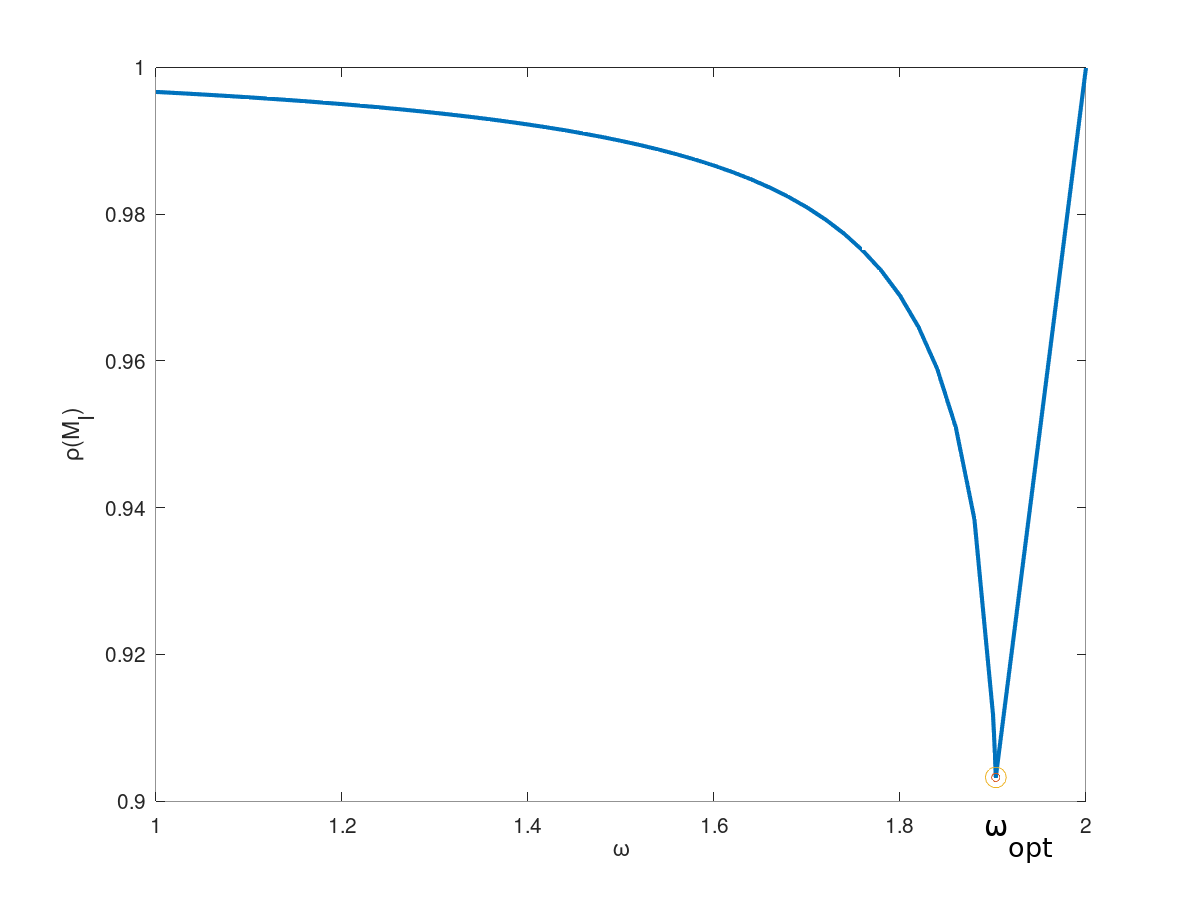
\includegraphics[width=0.6\linewidth]{omegaopt.png}
\end{figure}

\section{Método de gradiente (o del descenso mas rápido)}

Cuando trabajamos con matrices definidas positivas es posible reemplazar el problema:
$$
\mbox{(P1) Hallar $\xb\in \R^n$ tal que
}\,\Ab\xb=\bb
$$
por un problema de minimización  asociado a la función $J(\zb)=\frac{1}{2}\zb^*\Ab\zb-\zb^*\bb$:
$$
\mbox{(P2) Hallar $\xb\in \Rn$ tal que}\, J(\xb)=
\min_{\yb\in \R^n}J(\yb)
$$
En efecto, supongamos que $\xb$ resuelve (P1). Calculamos para $\zb\ne\cero$
$$
h(t)=J(\xb+t\zb)= \frac{1}{2}(\xb+t\zb)^*\Ab(\xb+t\zb)-(\xb+t\zb)^*\bb=
$$
$$
\frac{1}{2}t^2\zb^*\Ab\zb+t\left(\zb^*\Ab\xb-\zb^*\bb\right) +\frac{1}{2}\xb^*\Ab\xb-\xb^*\bb
$$
y observamos que $h(t)$ resulta ser una cuadr\'atica en la variable $t$, con mínimo en
$$
t_m=\frac{\zb^*\Ab\xb-\zb^*\bb}{\zb^*\Ab\zb},
$$
pero por otro lado como $\Ab\xb=\bb$, debe ser $t_m=0$. Entonces
$$
J(\xb)=h(0)\le h(t)=J(\xb+t\zb)
$$
para todo $t$ entonces
$$
J(\xb)=\min_{\yb\in\Rn}J(\yb),
$$
lo que dice que $\xb$ resuelve $(P2)$.
Recíprocamente: si $\xb$ es tal que 
$$
J(\xb)=\min_{\yb\in\Rn}J(\yb),
$$
repetimos la cuenta anterior y vemos que el mínimo de $h(t)$ está en $t=0$ lo que dice que
$$0=\frac{\zb^*\Ab\xb-\zb^*\bb}{\zb^*\Ab\zb}
$$
es decir
$$
\zb^*(\Ab\xb-\bb)=0,
$$
para todo $\zb\neq \cero$, lo que indica que \footnote{Tomando, por ejemplo, $\zb=\Ab\xb-\bb$.}
$$
\Ab\xb-\bb=\cero,
$$
es decir
$$
\Ab\xb=\bb.
 $$
 y entonces $\xb$ resuelve $(P1)$.

Ejemplo en $\R^2$: $
\Mb=\begin{pmatrix}
     5&2\\
     2&4
    \end{pmatrix}
$, $
\bb=\begin{pmatrix}
     1\\
     0
    \end{pmatrix}
$,
$$
\Mb\xb=\bb
$$
$\xb=\begin{pmatrix}
    1/4\\
    -1/8
     \end{pmatrix}
$
$$
J(x_1,x_2)=5/2x_1^2+2x_2^2+2x_1x_2-x_1
$$
En la Figura \ref{fig:curvasdeJ} vemos las curvas de nivel de $J$ y el punto $\xb$ (en rojo) solución del sistema. 


\begin{figure}[h]
\centering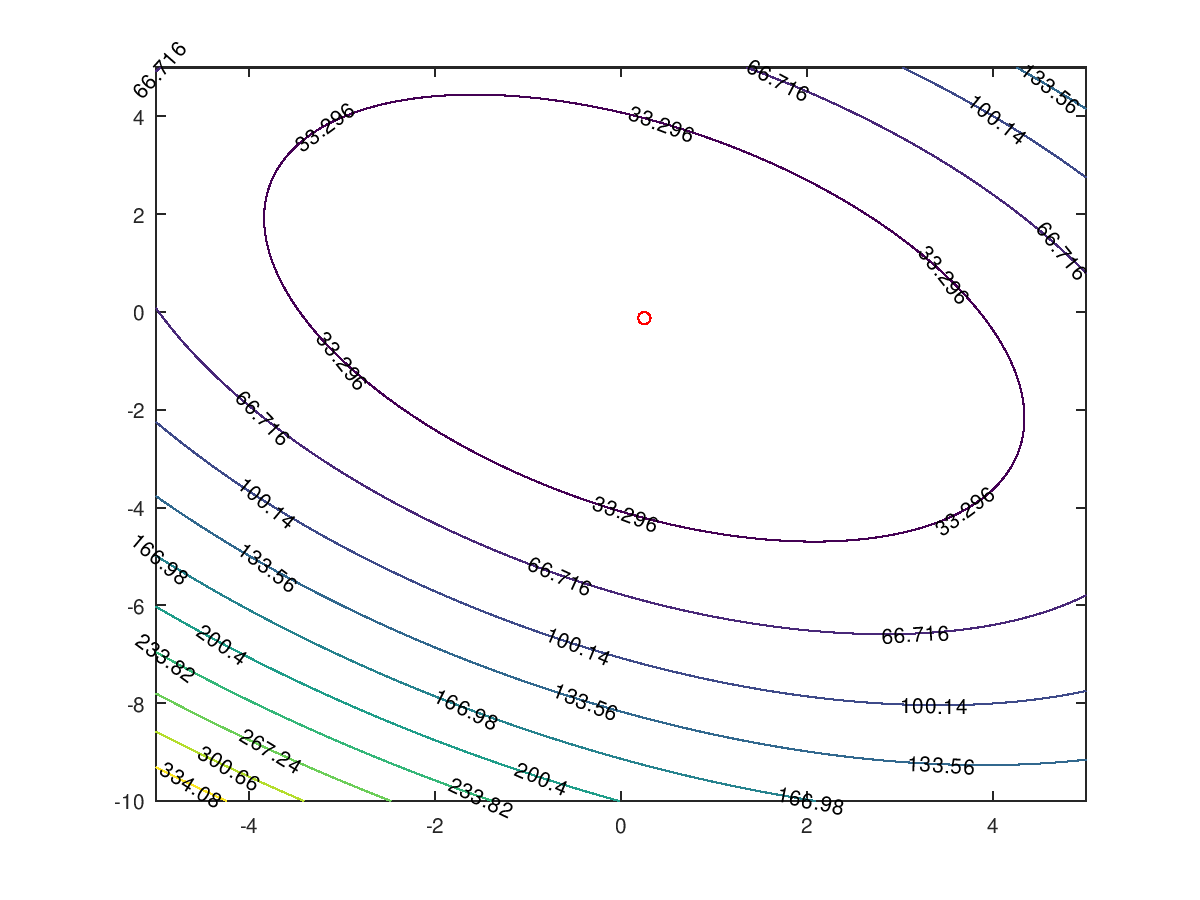
\includegraphics[width=0.4\linewidth]{curvasnivel.png}
\label{fig:curvasdeJ}
\caption{Curvas de nivel de $
J(x_1,x_2)=5/2x_1^2+2x_2^2+2x_1x_2-x_1
$.}
\end{figure}

Podemos comenzar simplificando el problema de minimización en $\R^n$ y llevarlo a uno que sea iterativo en $\R$. Este es un m\'etodo de busqueda por líneas. Dado $\xb_i$ elegimos una dirección de búsqueda $\zb_i$ y un escalar $\lambda_i$ tal que
$$
\xb_{i+1}=\xb_i+\lambda_i\zb_i.
$$
En un caso general quisieramos $\lambda_i$ tal que
$$
J(\xb_{i}+\lambda_i\zb_i )=\min_{t\in \R}J(\xb_i+t\zb_i),
$$

lo que nos llevaría a resolver
$$
0=\frac{dJ(\xb_{i}+t\zb_i )}{dt}=\nabla J(\xb_{i}+t\zb_i )^*\zb_i.
$$
En el caso que nos interesa ya sabemos despejar $\lambda_i$:
$$
\lambda_i=\frac{\zb_i^*(\Ab\xb_i-\bb)}{\zb_i^*\Ab\zb_i}=
\frac{\zb_i^*\rb_i}{\zb_i^*\Ab\zb_i}
$$
donde $\rb_i=\Ab\xb_i-\bb$ es el residuo.

Este método no nos sugiere como elegir el vector de búsqueda $\zb_i$ en cada paso. Una forma natural es utilizar la dirección de mayor decrecimiento\footnote{O crecimiento que son opuestas.} de la función $J$ en el punto $\xb_i$ : $\nabla J(\xb_i)=\Ab\xb_i-\bb=\rb_i$. Esto da lugar al método del gradiente o del descenso más rápido:
$$
\xb_{i+1}=\xb_i+\frac{\rb_i^*\rb_i}{\rb_i^*\Ab\rb_i}
\rb_i.
$$


El proceso anterior puede converger muy lentamente. 
En cada paso minimizamos (de forma exacta en aritmética exacta) a lo largo de la recta $\xb_i+\lambda \zb_i$.

Una mejora sustancial sería intentar minimizar el paso $i$ $$
J(\xb_{i+1})=\min_{\yb\in \langle \zb_0,\cdots\zb_i \rangle + x_0}J(\yb)
$$
que claramente daría un algoritmo que finaliza\footnote{Al menos en aritmética exacta.} en a lo sumo $n$ pasos. Ese algoritmo lo estudiamos en la siguiente sección.
\section{Gradiente Conjugado}
Observemos, antes de continuar, que una matriz (simétrica o Hermitiana) definida positiva define un producto interno a través de la operación\footnote{Dejamos como ejercicio esta afirmación.}
$$
\xb^T\Ab\yb.
$$
En particular este producto posee la siguiente norma asociada 
$$
\|\xb\|_A=\sqrt{\xb^T\Ab\xb}.
$$
Teniendo esta norma definida probamos lo siguiente.
\tcc
\begin{lema}
Supongamos que las direcciones de búsqueda son $\Ab$ ortogonales (i.e. $\zb_i^T\Ab\zb_j=0$) y en cada paso $\lambda_i$ se elige para minimizar sobre la línea correspondiente. Entonces
$$
\min_{\xb_i+\langle \zb_i\rangle}J(\yb)=J(\xb_{i+1})=\min_{\yb\in \xb_0+\langle \zb_0,\zb_1,\cdots,\zb_i \rangle} J(\yb)
$$
\end{lema}
\etcc
\begin{proof}
 Sea $W_{i+1}=\langle \zb_0,\zb_1,\cdots,\zb_i \rangle$ y tomo $\zb\in \xb_0+W_{i+1}$ arbitrario. Por construcción, se puede escribir 
 $$\zb=\yb+t\zb_i$$ con $\yb\in \xb_0+ W_i=\xb_0+\langle \zb_0,\zb_1,\cdots,\zb_{i-1} \rangle$. 
 
 Observamos que  
  $$
 \min_{\zb\in \xb_0+W_{i+1}}J(\zb)=\min_{\yb\in\xb_0+W_{i},t \in \R} J(\yb+t \zb_i) 
 $$

 $$
 $$
Escribimos 
$$
J(z)=J(\yb+t\zb_i)=\frac{1}{2}t^2\zb_i^T\Ab\zb_i+t\left(\zb_i^T\Ab\yb-\zb_i^*\bb\right) +\frac{1}{2}\yb^*\Ab\yb-\yb^*\bb
$$
pero, usando que $\zb_i^T\Ab\zb_j=0$ 
$$
\zb_i^T\Ab\yb=\zb_i^T\Ab\xb_0=\zb_i^T\Ab\xb_i
$$
$$
J(\yb+t\zb_i)=\left(\frac{1}{2}t^2\zb_i^T\Ab\zb_i+t\left(\zb_i^T\Ab\xb_i-\zb_i^T\bb\right)\right) +\frac{1}{2}\yb^T\Ab\yb-\yb^T\bb
$$
de donde resulta que 
para minimizar en $\zb$ basta minimizar ambos términos: el primero en $t\in \R$ el segundo en $\yb\in W_i$. Pero el $t$ óptimo es justamente $\lambda=\frac{\zb_i^T\Ab\rb_i}{\zb_i^T\Ab\zb_i}$ provisto por nuestro método. En definitiva
  el resultado sale por inducción.
\end{proof}

\tccdefi
\begin{center}Las direcciones $\Ab$ ortogonales suelen llamarse conjugadas
\end{center}
\etcc
Queremos un método que minimice sobre direcciones conjugadas (y no sea costoso)

Idea: A-ortogonalizar los residuos
\begin{itemize}
 \item $\zb_0=\rb_0$
 \item $\zb_i=\rb_i-\sum_{j=0}^{i-1}\frac{\zb_j^T\Ab\rb_i}{\zb_j^T\Ab\zb_j}\zb_j$
\end{itemize}
 


Vale lo siguiente
\begin{itemize}
 \item $\langle \zb_0, \zb_1\cdots ,\zb_i\rangle =\langle \rb_0, \rb_1\cdots ,
 \rb_i\rangle$
\item $\rb_i^T\rb_j=0$, pues $J(\xb_i+t\rb_j)$ tiene un mínimo en $t=0$, si $0\le j<i$. Luego derivando y evaluando en $t=0$
$$
0=\rb_j^T(\Ab\xb_i-\bb)=\rb_j^T\rb_i.
$$
\item Existe $m\le n$ tal que 
$$
\xb_0\neq \xb_1\neq \cdots \neq \xb_m= \xb
$$
$$
W_{0}\subsetneq W_1\subsetneq \cdots \subsetneq W_m
$$
 
\item Para todo $1\le i\le m$, $\{ \zb_0,\zb_1\cdots \zb_{i-1}\}$ (resp. $\{ \rb_0,\rb_1\cdots \rb_{i-1}\}$) es una base $A$ ortogonal (resp. ortogonal) de $W_i$.
 \item $\zb_i^T\rb_i=\rb_i^T\rb_i$. Pues 
 $\zb_i=\rb_i-\sum_{j=0}^{i-1}\frac{\zb_j^T\Ab\rb_i}{\zb_j^T\Ab\zb_j}\zb_j$ y entonces 
 $$\rb_i^T\zb_i=\rb_i^T\rb_i-\sum_{j=0}^{i-1}\frac{\zb_j^T\Ab\rb_i}{\zb_j^T\Ab\zb_j}\rb_i^T\zb_j=\rb_i^T\rb_i$$
 pues para cada $j\le i-1$,
 $\zb_j\in W_i=\langle \rb_0,\cdots,\rb_{i-1}\rangle$, $\rb_i^T\zb_j=0.$ 
 \end{itemize}


 Queremos hallar las direcciones de búsqueda sin hacer Gram-Schmidt (o sea mas rápido)

Escribamos $\zb_i$ en la base de los residuos (ortogonales), 
$$
\zb_i=\sum_{j=0}^{i}\frac{\zb_i^T\rb_j}{\rb_j^T\rb_j}\rb_j,
$$
ya vimos que
$\zb_i^T\rb_i=\rb_i^T\rb_i$
pero además
$\zb_i^T(\rb_i-\rb_l)=\zb_i^T\Ab(\xb_i-\xb_l)=0$ porque $\xb_i-\xb_l\in W_i$ y $\zb_i$ es $A$ ortogonal a $W_i$.
$$
\zb_i=\sum_{j=0}^{i}\frac{\zb_i^T\rb_j}{\rb_j^T\rb_j}\rb_j=\sum_{j=0}^{i}\frac{\rb_i^T\rb_i}{\rb_j^T\rb_j}\rb_j=\rb_i + \rb_i^T\rb_i\sum_{j=0}^{i-1}\frac{\rb_j}{\rb_j^T\rb_j},
$$
como la ultima sumatoria permite escribir recursivamente las direcciones de búsqueda

$$
\rb_i + \rb_i^T\rb_i\sum_{j=0}^{i-1}\frac{\rb_j}{\rb_j^T\rb_j}=\rb_i + \frac{\rb_i^T\rb_i}{\rb_{i-1}^T\rb_{i-1}}\left( \rb_{i-1}+\rb_{i-1}^T\rb_{i-1}\sum_{j=0}^{i-2}\frac{\rb_j}{\rb_j^T\rb_j}\right)
$$
entonces
$$
\zb_i=\rb_i+\frac{\rb_i^T\rb_i}{\rb_{i-1}^T\rb_{i-1}}\zb_{i-1}
$$
los residuos  pueden obtenerse de 
$$\xb_{i+1}=\xb_i+\lambda \zb_i$$ 
$$
\rb_{i+1}=\rb_i+\lambda_i\Ab\zb_i
$$

Tomo $\xb_0$, calculo $\rb_0$ asigno $\zb_0=\rb_0$

\noindent { for i=0... }
\begin{itemize}
 \item $\lambda_i=\frac{\rb_i^T\rb_i}{\zb_{i}^T\Ab\zb_i}$
 \item $\xb_{i+1}=\xb_{i}+\lambda_i \zb_i$
 \item $\rb_{i+1}=\rb_i+\lambda_i\Ab\zb_i$
\item $
\zb_{i+1}=\rb_{i+1}+\frac{\rb_{i+1}^T\rb_{i+1}}{\rb_{i}^T\rb_{i}}\zb_{i}
$

\end{itemize}
end

Aplicado a nuestro caso de ejemplo: para un error de orden $10^{-4}$ tarda $0.057$ segundos...

Para estudiar el error del GC notemos
$$
W_i=\langle \rb_0, \Ab\rb_0, \cdots \Ab^{i-1}\rb_0\rangle
$$
lo cual se ve por inducción. Si $i=1$ es cierto, y asumiendo que vale para $i$ queremos ver que vale para $i+1$. Para eso vemos que basta con ver que 
$$
W_{i+1}\subset
\langle \rb_0, \Ab\rb_0, \cdots \Ab^{i}\rb_0\rangle
$$
puesto que $dim(W_{i+1})=i+1$

Asumiendo entonces que   
$$W_{i}\ni \rb_{i-1},\zb_{i-1}\in \langle \rb_0, \Ab\rb_0, \cdots ,\Ab^{i-1}\rb_0\rangle$$



se tiene que  $\rb_{i}=\rb_{i-1}-\lambda_{i-1}\Ab\zb_{i-1}\in \langle \rb_0, \Ab\rb_0, \cdots ,\Ab^{i}\rb_0\rangle$
que es lo que queríamos ver.


Estos subespacios se llaman de Krylov. A veces se escribe
$\langle \bb, \Ab\bb, \cdots ,\Ab^{i}\bb\rangle$


$$\langle \rb_0, \Ab\rb_0, \cdots \Ab^{i-1}\rb_0\rangle=\{ p(\Ab)\rb_0: p\in P_{i-1}[x]\}=$$
$$=\{ q(\Ab)(\xb-\xb_0): q\in P_{i}[x],\ q(0)=0\}$$

Va a resultar cómodo estudiar el error en la norma $\|\cdot\|_A$: es decir quiero acotar 
$$
\|\xb-\xb_i\|_{A}$$

Como $\rb_i$ es ortogonal a $W_i$, $\xb-\xb_i
$ es $A$ ortogonal a $W_i$
$$
\|\xb-\xb_i\|_{A}=\inf_{\yb\in W_i}\|\xb-\xb_i-\yb\|_{A}
$$
como $\xb_0-\xb_i\in W_i$
$$
\|\xb-\xb_i\|=\inf_{\yb\in W_i}
\|\xb-\xb_0-\yb\|_{A}
=$$

$$
=\inf_{q\in P_{i}[x],q(0)=0}\|\xb-\xb_0-q(\Ab)(\xb-\xb_0)\|_{A}
=$$
$$
=\inf_{p\in P_i[x],p(0)=1}\|p(\Ab)(\xb-\xb_0)\|_{A}
\le$$
$$
\inf_{p\in P_i[x],p(0)=1}\|p(\Ab)\|_{A}\|(\xb-\xb_0)\|_{A}
$$

pero
$$
\|p(\Ab)\|_A^2=\sup_{\xb\neq\cero}\frac{\|p(\Ab)\xb\|_A^2}{\|\xb\|_A^2}=
$$
$$=\sup_{\xb\neq\cero}\frac{(p(\Ab)\xb)^T\Ab (p(\Ab)\xb)}{\xb^T\Ab\xb}=\sup_{\xb\neq\cero}\frac{\xb^T p(\Ab)^T\Ab p(\Ab)\xb}{\xb^T\Ab\xb}=
$$
$$
=\sup_{\xb\neq\cero}\frac{\xb^T\Ab^{1/2} p(\Ab)^T p(\Ab)\Ab^{1/2}\xb}{\xb^T\Ab^{1/2}\Ab^{1/2}\xb}=sup_{\yb\neq\cero}\frac{\yb^T p(\Ab)^T p(\Ab)\yb}{\yb^T\yb}
=$$
$$
=sup_{\yb\neq\cero}\frac{ \|p(\Ab)\yb\|_2^2}{\|\yb\|^2_2}
=\|p(\Ab)\|_2^2=\rho(p(\Ab))^2\le \max_{\lambda\in [\lambda_1,\lambda_n]}p(\lambda)^2$$

En definitiva

$$
\|p(\Ab)\|_A\le  \max_{x\in [\lambda_1,\lambda_n]}|p(x)| 
$$
y hay que acotar
$$
\inf_{p\in P_i[x],p(0)=1}\max_{x\in [\lambda_1,\lambda_n]}|p(x)|
$$
esto, por suerte, lo estudió Chebyshev.

En el intervalo $[-1,1]$ los polinomios de Chebyshev son
$$
T_0(x)=1,T_1(x)=x,T_2(x)=2x^2-1,\cdots 
$$
en general
$$
T_{n+1}(x)=2T_{n}(x)-T_{n-1}(x)
$$

Para $x\in [-1,1]$, $|T_n(x)|\le 1$ 

(de hecho 
en ese rango $T_n(x)=\cos(n\cos^{-1}(x))$)

para $|x|\ge 1$
$$
T_n(x)=\frac12\left((x+\sqrt{x^2-1})^n+ (x-\sqrt{x^2-1})^n\right)
$$


El polinomio $p(x)\in P_n[x]$ que minimimiza $\max_{x\in [\lambda_1,\lambda_n]}|p(x)|$ con la condición $p(0)=1$ es
$$
\frac{1}{T_n(\frac{\lambda_n+\lambda_1}{\lambda_1-\lambda_n})}T_n\left(\frac{2x-\lambda_n-\lambda_1}{\lambda_n-\lambda_1}\right)$$


$$
\inf_{p\in P_i[x],p(0)=1}\max_{x\in [\lambda_1,\lambda_n]}|p(x)|
\le \frac{2}{\left( \frac{\sqrt{\frac{\lambda_n}{\lambda_1}}+1}{\sqrt{\frac{\lambda_n}{\lambda_1}}-1}\right)^i+\left( \frac{\sqrt{\frac{\lambda_n}{\lambda_1}}-1}{\sqrt{\frac{\lambda_n}{\lambda_1}}+1}\right)^i}$$ 
es decir
$$
\inf_{p\in P_i[x],p(0)=1}\max_{x\in [\lambda_1,\lambda_n]}|p(x)|
\le 2\left(\frac{\sqrt{\kappa(\Ab)}-1}{\sqrt{\kappa(\Ab)}+1}\right)^i
$$
 
$$\|\xb-\xb_i\|_{A}\le 2\left(\frac{\sqrt{\kappa(\Ab)}-1}{\sqrt{\kappa(\Ab)}+1}\right)^i\|\xb-\xb_0\|_{A}$$

 
